%!TEX root = ../thesis.tex
%*******************************************************************************
%*********************************** First Chapter *****************************
%*******************************************************************************
\chapter{Introduction}  %Title of the First Chapter

\ifpdf
    \graphicspath{{Chapter1/Figs/Raster/}{Chapter1/Figs/PDF/}{Chapter1/Figs/}}
\else
    \graphicspath{{Chapter1/Figs/Vector/}{Chapter1/Figs/}}
\fi


%********************************** %First Section  **************************************

\newacro{cnn}[\textsc{Cnn}]{Convolutional neural network}

Deep Neural Networks (DNNs), are connectionist systems that learn to perform tasks by learning on examples without having a prior knowledge about the tasks. 
They easily scale to millions of data points and yet remain tractable to optimize with stochastic gradient descent.

Convolutional Neural Networks (CNNs), a variant of DNNs, have already surpassed human accuracy in the realm of image classification (e.g. \cite{he2016deep,simonyan2014very,krizhevsky2012imagenet}). Due to the capacity of \acp{cnn} to fit on a wide diversity of non-linear data points, they require a large amount of training data. This often makes \acp{cnn}s and Neural Networks in general, prone to overfitting on small datasets. The model tends to fit well to the training data, but are not predictive for new data. This often makes the Neural Networks incapable of correctly assessing the uncertainty in the training data and hence leads to overly confident decisions about the correct class, prediction or action.

Various regularization techniques for controlling over-fitting are used in practice namely early stopping, weight decay, L1, L2 regularizations and currently the most popular and empirically effective technique being \emph{dropout}~\cite{hinton2012improving}. 


\section{Problem Statement}

Despite Neural Networks architectures achieving state-of-the-art results in almost all classification tasks, Neural Networks still make over-confident decisions. A measure of uncertainty in the prediction is missing from the current Neural Networks architectures. Very careful training, weight control measures like regularization of weights and similar techniques are needed to make the models susceptible to over-fitting issues. 

We address both of these concerns by introducing Bayesian learning to a Convolutional Neural Networks that adds a measure of uncertainty and regularization in their predictions. 

\section{Current Situation}

Deep Neural Networks have been successfully applied to many domains, including sensitive domains like health-care, security, fraudulent transactions and many more. However, from a probability theory perspective, it is unjustifiable to use single point-estimates as weights to base any classification on.
On the other hand, Bayesian neural networks (NNs) are more robust to over-fitting, and can easily learn from small datasets. The Bayesian approach further offers uncertainty estimates via its parameters in form of probability distributions (see Figure \ref{fig:Scalar_Bayesian_Distribution}). At the same time, by using a prior probability distribution to integrate out the parameters, the average is computed across many models during training, which gives a regularization effect to the network, thus preventing overfitting.


Bayesian posterior inference over the neural network parameters is a theoretically attractive method for controlling overfitting; however, modelling a distribution over the kernels (also known as filters) of a \acp{cnn} has never been attempted successfully before, perhaps because of the vast number of parameters and extremely large models commonly used in practical applications.

Even with a small number of parameters, inferring model posterior in a Bayesian NN is a difficult task. Approximations to the model posterior are often used instead, with the variational inference being a popular approach. In this approach one would model the posterior using a simple \textit{variational} distribution such as a Gaussian, and try to fit the distribution's parameters to be as close as possible to the true posterior. This is done by minimising the Kullback-Leibler divergence from the true posterior. Many have followed this approach in the past for standard NN models \citep{hinton1993keeping,barber1998ensemble,graves2011practical,blundell2015weight}.
But the variational approach used to approximate the posterior in Bayesian NNs can be fairly computationally expensive -- the use of Gaussian approximating distributions increases the number of model parameters considerably, without increasing model capacity by much. \citet{blundell2015weight} for example use Gaussian distributions for Bayesian NN posterior approximation and have doubled the number of model parameters, yet report the same predictive performance as traditional approaches using dropout. This makes the approach unsuitable for use with \acp{cnn}s as the increase in the number of parameters is too costly.

\begin{figure}[H]
\begin{center}
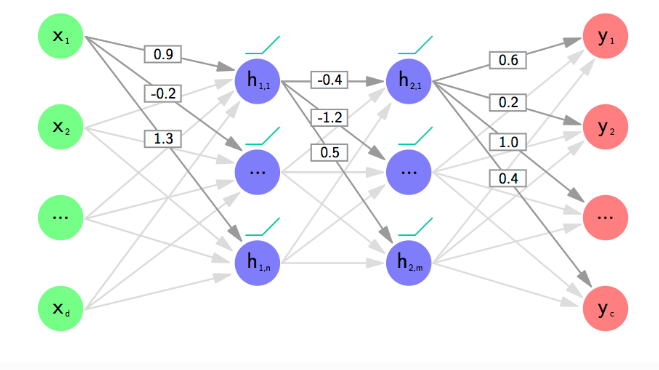
\includegraphics[height=.28\textheight]{Chapter1/Figs/weights.png}
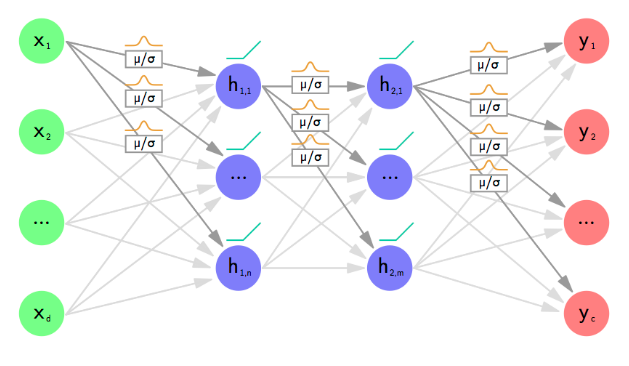
\includegraphics[height=.28\textheight]{Chapter1/Figs/distribution.png}
\label{fig:Scalar_Bayesian_Distribution}
\caption{Top: Each filter weight has a fixed value, as in the case of frequentist Convolutional Networks. Bottom: Each filter weight has a distribution, as in case of Bayesian Convolutional Networks. \cite{Gluon}}
\end{center}
\end{figure}

\section{Our Hypothesis}
\newline We build our Bayesian \ac{cnn} upon \textit{Bayes by Backprop} \cite{graves2011practical,blundell2015weight}. The exact Bayesian inference on the weights of a neural network is intractable as the number of parameters is very large and the functional form of a neural network does not lend itself to exact integration. So, we approximate the intractable true posterior probability distributions $p(w|\mathcal{D})$ with variational probability distributions $q_{\theta}(w|\mathcal{D})$, which comprise the properties of Gaussian distributions $\mu \in \mathbb{R}^d$ and $\sigma \in \mathbb{R}^d$, denoted $\mathcal{N}(\theta|\mu, \sigma^2)$, where $d$ is the total number of parameters defining a probability distribution. The shape of these Gaussian variational posterior probability distributions, determined by their variance $\sigma^2$, expresses an uncertainty estimation of every model parameter. \\ \\



\section{Our Contribution}
\newline The main contributions of our work are as follows: 
\begin{enumerate}
    \item We present how \textit{Bayes by Backprop} can be efficiently applied to \acp{cnn}. We, therefore, introduce the idea of applying two convolutional operations, one for the mean and one for the variance.
    \item We show how the model learns richer representations and predictions from cheap model averaging.
    \item We empirically show that our proposed generic and reliable variational inference method for Bayesian \acp{cnn} can be applied to various \ac{cnn} architectures without any limitations on their performances. 
    \item We examine how to estimate the aleatoric and epistemic uncertainties and empirically show how the uncertainty can decrease, allowing the decisions made by the network to become more deterministic as the training accuracy increases. 
    \item We also empirically show how our method typically only doubles the number of parameters yet trains an infinite ensemble using unbiased Monte Carlo estimates of the gradients. 
    \item We also apply L1 norm to reduce the trained parameters and perform model pruning to reduce the number of model parameters without a reduction in the model prediction accuracy. 
\end{enumerate} 
This work builds on the foundations laid out by Blundell et al. \cite{blundell2015weight}, who introduced \textit{Bayes by Backprop} for feedforward neural networks. Together with the extension to recurrent neural networks, introduced by Fortunato et al. \cite{fortunato2017bayesian}, \textit{Bayes by Backprop} is now applicable on the three most frequently used types of neural networks, i.e., feedforward, recurrent, and convolutional neural networks.


%\nomenclature[z-cif]{$CIF$}{Cauchy's Integral Formula}                                % first letter Z is for Acronyms 
